\def\year{2018}\relax
%File: formatting-instruction.tex
\documentclass[letterpaper]{article} %DO NOT CHANGE THIS
\usepackage{aaai18}  %Required
\usepackage{times}  %Required
\usepackage{helvet}  %Required
\usepackage{courier}  %Required
\usepackage{url}  %Required
\usepackage{graphicx}  %Required
\usepackage{enumitem}
\usepackage{lipsum}
\setlist[enumerate]{itemsep=0mm}
\frenchspacing  %Required
\setlength{\pdfpagewidth}{8.5in}  %Required
\setlength{\pdfpageheight}{11in}  %Required
%PDF Info Is Required:
\pdfinfo{
	/Title (Transfer Learning for Traffic Speed Prediction: A Preliminary Study)
	/Author (Bill Y. Lin, Frank F. Xu, Eve Q. Liao, Kenny Q. Zhu)}

\title{Transfer Learning for Traffic Speed Prediction: A Preliminary Study}

% The \author macro works with any number of authors. There are two
% commands used to separate the names and addresses of multiple
% authors: \And and \AND.
%
% Using \And between authors leaves it to LaTeX to determine where to
% break the lines. Using \AND forces a line break at that point. So,
% if LaTeX puts 3 of 4 authors names on the first line, and the last
% on the second line, try using \AND instead of \And before the third
% author name.
\author{
	Bill Y. Lin\thanks{The first two authors contribute equally.}, 
	Frank F. Xu\footnotemark[1], Eve Q. Liao, 
	Kenny Q. Zhu
	\\[0.5ex]
	{\{yuchenlin, frankxu, liaoqz\}@sjtu.edu.cn, kzhu@cs.sjtu.edu.cn}\\[0.5ex]
	Department of Computer Science and Engineering\\[0.5ex]
	Shanghai Jiao Tong University, Shanghai, China
}

\usepackage{amsmath,amsfonts,amsthm}
\usepackage{color}
\usepackage{array}
\usepackage{epsfig}
\usepackage{caption}
\usepackage{subcaption}
\usepackage{array}
\usepackage{ragged2e}
\usepackage{pbox}

\usepackage[ruled,vlined,boxed,linesnumbered]{algorithm2e}
\SetAlFnt{\small}
\SetAlCapFnt{\small}
\SetAlCapNameFnt{\small}

\newcolumntype{P}[1]{>{\RaggedRight\hspace{0pt}}p{#1}}
\newcolumntype{L}[1]{>{\raggedright\let\newline\\\arraybackslash\hspace{0pt}}m{#1}}
\newcolumntype{C}[1]{>{\centering\let\newline\\\arraybackslash\hspace{0pt}}m{#1}}
\newcolumntype{R}[1]{>{\raggedleft\let\newline\\\arraybackslash\hspace{0pt}}m{#1}}


\newcommand{\secref}[1]{Section \ref{#1}}
\newcommand{\figref}[1]{Figure \ref{#1}}
\newcommand{\eqnref}[1]{Eq. (\ref{#1})}
\newcommand{\tabref}[1]{Table \ref{#1}}
\newcommand{\exref}[1]{Example \ref{#1}}
\newcommand{\algref}[1]{Algorithm \ref{#1}}
\newcommand{\socvec}{SocVec}
\newcommand{\argmin}{\operatornamewithlimits{argmin}}
\newcommand{\argmax}{\operatornamewithlimits{argmax}}
\newtheorem{example}{Example}
\newtheorem{lemma}{Lemma}
\newtheorem{definition}{Definition}
\newcommand{\cut}[1]{}
\newcommand{\li}{\uline{\hspace{0.5em}}}


%\author{
%  David S.~Hippocampus\thanks{Use footnote for providing further
%    information about author (webpage, alternative
%    address)---\emph{not} for acknowledging funding agencies.} \\
%  Department of Computer Science\\
%  Cranberry-Lemon University\\
%  Pittsburgh, PA 15213 \\
%  \texttt{hippo@cs.cranberry-lemon.edu} \\
  %% examples of more authors
  %% \And
  %% Coauthor \\
  %% Affiliation \\
  %% Address \\
  %% \texttt{email} \\
  %% \AND
  %% Coauthor \\
  %% Affiliation \\
  %% Address \\
  %% \texttt{email} \\
  %% \And
  %% Coauthor \\
  %% Affiliation \\
  %% Address \\
  %% \texttt{email} \\
  %% \And
  %% Coauthor \\
  %% Affiliation \\
  %% Address \\
  %% \texttt{email} \\
%}

\begin{document}
\maketitle

\begin{abstract}
Traffic speed prediction can benefit a wide range of IoT applications in intelligent transportation and smart city. 
Recent supervised machine learning approaches heavily leverage vast amount of historical time-series data. 
Consequently, they degrade dramatically in the areas where collecting a large traffic data is not quite feasible.
With the aim of predicting the traffic speed of such urban areas, 
we propose a transfer learning framework that exploits historical data of some other data-abundant areas by utilizing various spatio-temporal semantic features. 
Experimental results show that classic regression models and our proposed kernel regression model can achieve competitive performance comparing to baseline methods that heavily rely on the historical data of target areas.
\end{abstract}
\section{Introduction}
Traffic speed prediction is a challenging problem and has various downstream applications of Internet of Things (IoT), many of which are fundamental to intelligent transportation systems and smart city, such as
congestion management, urban planning, vehicle routing, etc.~\cite{Pan2012,Xu2015,Mchugh2015}.

Most existing machine learning approaches heavily rely on the vast amount of historical data for the areas being predicted~\cite{Ren2014,Clark2003Traffic}.
However, accurate and reliable historical traffic data collected from road sensors is very expensive and available in urban areas where the government can afford the large cost.
Consequently, most state-of-the-art time-series based models cannot be applied directly on areas where little traffic data is available.

Another disadvantage of most existing approaches is that they only focus on temporal features and do not explicitly utilize semantic features from spatio-temporal patterns~\cite{yao2017short,lin2017road},
which benefit many practical applications of urban computing~\cite{zheng2014urban}.
Research on extracting such effective spatial features for traffic speed prediction is almost missing from the literature. 

The preliminary study aims to answer this research questions:
\textit{{{How can we exploit the data of data-abundant areas to predict traffic speed for areas without traffic data through their semantic spatio-temporal features?}}}
To the best of our knowledge, we are among the first to study transfer learning for traffic speed prediction~\cite{xu2016cross}.
The contributions of this paper are as follows: 
\begin{itemize}
	\item We extract various spatial features in multiple levels and combine them with temporal features to support this transfer learning scenario, which also improves the transparency of prediction models. 
	\item Based on the features, we propose a novel clustering-based transfer learning model. Experimental results show that proposed model perform competitively with classic regression methods, but using only distant supervision.
\end{itemize}
%1) Our proposed transfer learning~\cite{Pan:Survey} approach supports many classic regression models. 

%	\item We also built a preliminary immature framework based on the idea of Generative Adversarial Networks to capture the dependency across the neighboring road segments by learning traffic data as images. 

%\section{Related Work}
%In the following sections, we will first talk about the dataset we are interested in and how we extracted spatial features from multiple data sources.
%Then, we will introduce our framework in detail and our experiments. 
%Finally, we would like to talk our preliminary attempts to learn traffic data as images and utilize the idea of Generative Adversarial Networks to generate the joint prediction results. 

\section{Transfer Learning Scenario}
%In this section, we define our problem in a mathematically.
Consider we have a set of $n$ road segments with traffic speed sensors. 
At any given time $t$, 
each sensor $i$ provides a traffic speed reading at this current time, denoted as $v_i[t]$.
Traffic speed prediction problem is to predict a future traffic speed like $v_i[t+h]$ at a previous time $t$. 
Most models utilize historical traffic data to predict the future speed of the same areas. 
However, when historical data such as $v_i[1:t]$ is not available, it is infeasible for them to predict. 

In this scenario, a transfer learning~\cite{Pan:Survey} approach is supposed to exploit the data of some \textit{source areas} $\mathcal{S}$ to build a prediction model for other \textit{target} areas $\mathcal{T}$, where there is little traffic speed data.
Mathematically, given $\{v_i[1:t]|i\in \mathcal{S}\}$, a transfer learning model is expected to be able to predict $\{v_j[1:t]|j\in \mathcal{T}\}$.




\section{Traffic Estimates Dataset}
In this section, we briefly introduce a public dataset named \textit{UIUC New York City Traffic Estimates}\footnote{\url{https://publish.illinois.edu/dbwork/open-data/}}, on which we extract spatial features and conduct our following experiments.
This dataset covers 700 million trips from 2010 to 2013 in New York City. 
It contains accurate hourly traffic speed measurement for almost all individual links of the NYC road networks.
Specific data format is described as follows:
\begin{enumerate}
	\item the road network is represented as a directed graph composed of \textit{nodes} and \textit{links}; 
	\item each \textit{node} is an intersection of the road network, with multiple properties like latitude and longitude;  
	\item each directed \textit{link} is a small road segment connecting two such nodes;   
	\item generally, a real street consists of multiple links;
	two-way streets are often represented as two directed links with opposite directions; 
	\item each row of the traffic speed data is the average traffic speed of a particular link at a particular hour.
\end{enumerate}
To evaluate transfer learning approaches, we split the road network into five different areas as shown in Table~\ref{tab:regions}.
%\footnote{The ``link\_num'' represents the number of the links in each region; 
%	the ``travel\_time\_num'' represents the number of the links in each region; 
%	the ``num\_trips\_sum'' represents the sum of the number of the trips involving all links in each region; }

\begin{table}[t]
	\centering
	\small
	\caption{Statistics of five areas in New York City}
	\label{tab:regions}
	\begin{tabular}{|c|c|c|c|c|c|}
		\cline{1-6}
		~& {Hudson}  & {Manhattan}  & {Brooklyn}  & {Bronx}    & {Queens}    \\ \hline
		\#link           & 730     & 8,578       & 7,790      & 2,113     & 8,173      \\ \hline
		%		travel   & 4949074 & 4450541890 & 241506751 & 15451922 & 412756499 \\ 
		%		\#trips\_sum & 477,596  & 52,394,074   & 24,121,488  & 5,002,542  & 20,531,664  \\ \hline
		\#trips\_sum & 477k  & 52m  & 24m & 5m  & 20m  \\ \hline
	\end{tabular}
\end{table}



\section{Spatiotemporal Features}
In this section, we discuss the proposed spatial features extracted from OpenStreetMap\footnote{\url{https://www.openstreetmap.com}} and temporal features that act as fundamental components of our proposed transfer learning approach. 
The proposed spatial features capture the traffic-related geographical characteristics for each link in road networks.

\subsection{Basic Information Features} 
An example of extracting the basic information for a particular link is shown in Figure~\ref{fig:basic}.
We have 5 features for representing the basic information of each link: 
\texttt{length}, \texttt{\#begin\_node\_in\_links}, \texttt{\#begin\_node\_out\_links}, \texttt{\#end\_node\_in\_links} and \texttt{\#end\_node\_out\_links}.
For each link, the \texttt{length} is the real distance between the begin and the end node of this link. 
The other 4 features represent the number of \textit{in} and \textit{out} links connected to both nodes of a link, which may provide information about crossroads or one-ways.

\begin{figure}[th]
	\centering
	\includegraphics[width=0.4\textwidth]{figures/basic.pdf}
	\caption{An example for extracting basic information features.}
	\label{fig:basic}
\end{figure}
\subsection{Road Density Features}
Additionally, we believe traffic speed is highly relevant to road density, which can be measured by the number of neighboring nodes and links within the same area.
To be more specific and capture the sensitivity about directions, we compute road density respectively for each end in terms of the density of neighboring node , and the density of neighboring in and out link,  according to three radius (100/300/500m), as shown in Figure~\ref{fig:road_density}.
%The nodes in the range of 100, 300 and 500 meters are marked as blue. The in/out links of these nodes are part of link features.
Consequently, we have $2 \times 3 \times 3 = 18$ road density features in total.
%
\begin{figure}[t]
	\centering
	\includegraphics[width=0.35\textwidth]{figures/roaddensity.pdf}
	\caption{An example of extracting the road density features with three different radius. The origin is begin/end node of a certain link, and each blue circle is a link intersection.}
	\label{fig:road_density}
\end{figure}


\subsection{Categorical POI Density Features}
Points of interest (POI) are specific locations that people may find useful or interesting, such as restaurants, shopping halls, parks, etc.
Since such places are very influential to the traffic, we query nearby POIs\footnote{The 11 major POI types we consider are \{\textit{Eat, Drink, Going Out, Sights \& Museums, Transport, Accommodation, Shopping, Business \& Services, Facilities, Facility, Administrative Areas/Buildings, Natural or Geographical}\}. } 
for each node with three different radius (100/300/500m) using HERE Places API\footnote{\url{https://developer.here.com/documentation/places/topics/introduction.html
}}. 
Figure~\ref{fig:poi} shows such an example for extract \textit{road density} features and\textit{ POI density features}. 

\begin{figure}[t]
	\centering
	\includegraphics[width=0.35\textwidth]{figures/poi.pdf}
	\caption{{An example for extracting POI Features. Different colors indicate different POI types.}}
	\label{fig:poi}
\end{figure}


\subsection{Temporal Features}
Our temporal feature is simply a distributed representation of the time information.
It is basically a concatenation of several one-hot vectors, 
where each vector represents the \textit{month}, the \textit{day} of a week, the \textit{hour} of a day and whether it is \textit{workday} respectively. 
%To sum up, the total number of spatial and temporal features is 89 and 44 correspondingly.


\section{Transfer Learning Approach}
Obtaining the above features for link and time,
we first apply several classic machine learning models for regression (Linear Regression, Neural Network model\footnote{A two-layer fully connected network model.}, Support Vector Regression).
They are trained on source areas with above-explored spatiotemporal features and then predict traffic condition on target areas as a test.
Afterwards, we present a novel transfer learning approach named CTMP.


%\subsection{CTMP: A Clustering-based Transfer Model }
We introduce our novel \textbf{C}lustering-based \textbf{T}ransfer \textbf{M}odel for \textbf{P}rediction  (CTMP), which first clusters links in both source and target areas based on their spatial features and then do time series based prediction for the target links based on neighboring source links with historical data.

\subsection{Intuition Behind the CTMP}
Our intuition behind CTMP is that given a link in target areas with spatial features, we can first find the most similar links in source areas and then leverage the source data to predict the speed of links in target areas.

The assumption here is that links with similar spatial features should also share similar traffic patterns.
However, simply clustering road links based on spatial features performs not very well in practice, because not all the features are equally important and the importances cannot be obtained in such an unsupervised way.
Therefore, we incorporate a regularization term in the distance metric for feature reduction and selection.\footnote{CTMP model can be seen as a combination of clustering and Nadaraya-Watson kernel regression.}

\subsection{Clustering with Regularized Distance Metric}
%\textit{Notations:} a prediction query instance about a link $l$ at the time $t$ is denoted as $(l,t)$; 
%the spatial feature vector for $l$ is denoted as  $s_l$, and the temporal feature vector of the time $t$ being predicted on the link $l$ is denoted as  $t_l$.
%The ground truth of the speed is denoted as $v_l[t]$.
We use the $s_i$ and $s_j$ to denote two spatial feature vectors of any two links $i$ and $j$ respectively.
We capture the distance between the two feature vectors by computing $\text{s\_dis}(i,j) = 1-\cos(s_i,s_j)$.
To regularize the time series similarities between two links, we add a regularization term $\text{t\_dis}(i,j)$, which has multiple options.
A desirable option is the DTW \cite{} similarities between the weekly HAM traffic speed series of the two links.
Thus, the total distance between two links can be regarded as follows, where $\lambda$ is a hyper parameter to control the weight of temporal distance:
$\text{dis}(i,j) =  \text{s\_dis}(i,j) + \lambda \text{t\_dis}(i,j) $.

With such supervision in the source area data,
we can use K-means as our clustering algorithm.
For each query instance $(l,t)$\footnote{The link $l$ has no historical data in the transfer scenario.}, we first find the closest $k$ neighboring source links with historical data $\{l_1,...l_k\}$.
We compute all the distances between them and the target link $l$ respectively, and obtain the set of spatial feature distances $\{\text{dis}(l,l_1),...,\text{dis}(l,l_k)\}$.
Also, we can get the predicted typical traffic speed for such neighboring links based on existing time-series models  at the time $t$: $\{y(l_1,t),...,y(l_k,t)\}$.
Finally, we can compute the predicted result for the query instance $(l,t)$ is:
$$ y(l,t) = \sum_{i=1}^k \left( \frac{\text{dis}(l,l_i)}{\sum_{j=1}^k \text{dis}(l,l_j)} 
y(l_i,t)
\right)$$ 


\section{Evaluation}
To evaluate the performance of our extracted features and proposed feature-based transfer regression models, we conduct a series of experiments to check both the performance of \textit{local transfer} and \textit{cross-region transfer}.
In this section, we first discuss the setup of our experiments, then the baseline methods and finally present the discussion of the experimental results.
\subsection{Experiment Setup}
We first split the data into training set and test set with respect to the time. 
Specifically, we first split the data in 2013 into two parts by timespan: Jan. - Jun. and Jul. - Dec.
Three scenarios are shown as follows:
\begin{enumerate}
	\item \textit{{No Transfer}} task is to predict the future speed  (the second half year) of a link with the historical (the first half year) data of the link.		
	\item \textit{{Local Transfer}} task is to consider the data in first half year as training data and second half year data as test data. 
	We train the models for each region with their data and test the models with the testing data in the same region. 
	\item \textit{{Cross-region Transfer}} task is to use a model trained on the first half year data of a source region to predict the traffic speed of another target region in the second half year.
	%For example, trained model on Brooklyn to predict the speed of Queens.
\end{enumerate}

\subsection{Baseline Methods}
We compare with the most representative time-series based regression models: ARIMA~\cite{ARIMA} and HAM~\cite{Pan2012}. 
%	\subsubsection{Auto-Regressive Integrated Moving Average (ARIMA)}
%%	ARIMA model is a generalization of an autoregressive moving average model. 
%%	Both of these models are fitted to time series data either to better understand the data or to predict future points in the series (forecasting). 
%	ARIMA models are applied on some cases where time series data shows evidence of non-stationarity and an initial differencing step (corresponding to the "integrated" part of the model) can be applied one or more times to eliminate the non-stationarity.
%	Prediction of the data for the time $t+1$  is:
%	$$ Y_{t+1} = \sum_{i=1}^p \alpha_i Y_{t-i+1}  + \sum_{i=1}^q \beta_i \epsilon_{t-i+1} + \epsilon_{t+1}$$
%	where $Y_t$ refers to a time series data. 
%	In the autoregressive component of this model, a linear weighted combination of previous data is calculated, where $p$ refers to the order of this model and $\alpha_i$ refers to the weight of $(t-i+1)$-th reading. 
%	As for the second part, the sum of weighted noise from the moving average model is calculated, where $\epsilon$ denotes the noise, $q$ refers to its order and $\beta_i$ represents the weight of $(t-i+1)$-th noise.
%	In our experiment, we trained ARIMA on the first half year to pick the parameters with best performance using 5-fold cross-validation.
%	


%\subsubsection{Historical Average Model (HAM)}
%HAM utilizes the average of previous speed data for the same time and same location to forecast the future data. 
%HAM is formulated as follows:
%$$  v (t_{d,w} +h ) = \frac{1}{|V(d,w)|} \sum _{s\in V(d,w)} \hspace{-8pt} v(s)$$
%where $V(d, w)$ refers to the subset of past observations that happened at the same time $d$ on the same weekday $w$. 
%Specifically, $d$ captures the daily effects while $w$ captures the weekly effects. 
%$7*24$ average regular speed tables for each link are derived from the data of first half year. 
%The model is evaluated by comparing using such tables. 
%%For example, if the traffic data of a link to be predicted is  at Monday 8:00AM, the ground true value is compared with the 'Monday' row, '8:00AM' column of its particular table.
%%\subsection{Our Methods}
%%	\subsubsection{Linear Regression Models}
%%		
%%	\subsubsection{Neural Network Models}
%%	\subsubsection{Support Vector Regression Models}
%%%	\subsection{}




\subsection{Experimental Results}

We first show the performance of HAM and ARIMA models on the \textit{No Transfer} Task with two metrics (RMSE and MAE) in Table~\ref{tbl:notransfer}.
We found that HAM performs substantially better than the ARIMA model with both metrics, 
which is probably due to the time interval in the dataset is one hour, quite longer than common time interval length for ARIMA model.
\begin{table}[th!]
	\small
	\centering
	\caption{\textit{No Transfer} performance of HAM and ARIMA}
	\label{tbl:notransfer}
	\begin{tabular}{|c|c|c|c|c|}
		\hline
		{}          & {\begin{tabular}[c]{@{}c@{}}HAM\\ \textit{RMSE}\end{tabular}} & {\begin{tabular}[c]{@{}c@{}}HAM\\ \textit{MAE}\end{tabular}} & {\begin{tabular}[c]{@{}c@{}}ARIMA\\ \textit{RMSE}\end{tabular}} & {\begin{tabular}[c]{@{}c@{}}ARIMA\\ \textit{MAE}\end{tabular}} \\ \hline
		{Total}     & 5.1802                                                  & 3.3152                                                & 6.7106                                                   & 4.2806                                                    \\ \hline
		{Hudson}    & 8.2871                                                 & 6.0331                                                & 11.5791                                                   & 8.8327                                                  \\ \hline
		{Manhattan} & 4.4532                                                 & 2.7495                                                & 5.2845                                                   & 3.1740                                                  \\ \hline
		{Brooklyn}  & 5.2661                                                 & 3.4681                                                & 6.8584                                                   & 4.6273                                                  \\ \hline
		{Bronx}     & 7.6168                                                 & 5.5544                                                 & 11.2118                                                   & 8.5488                                                  \\ \hline
		{Queens}    & 6.0233                                                 & 4.0720                                                & 8.2514                                                   & 5.7618                                                  \\ \hline
	\end{tabular}
\end{table}


\begin{figure*}[th!]
	\centering
	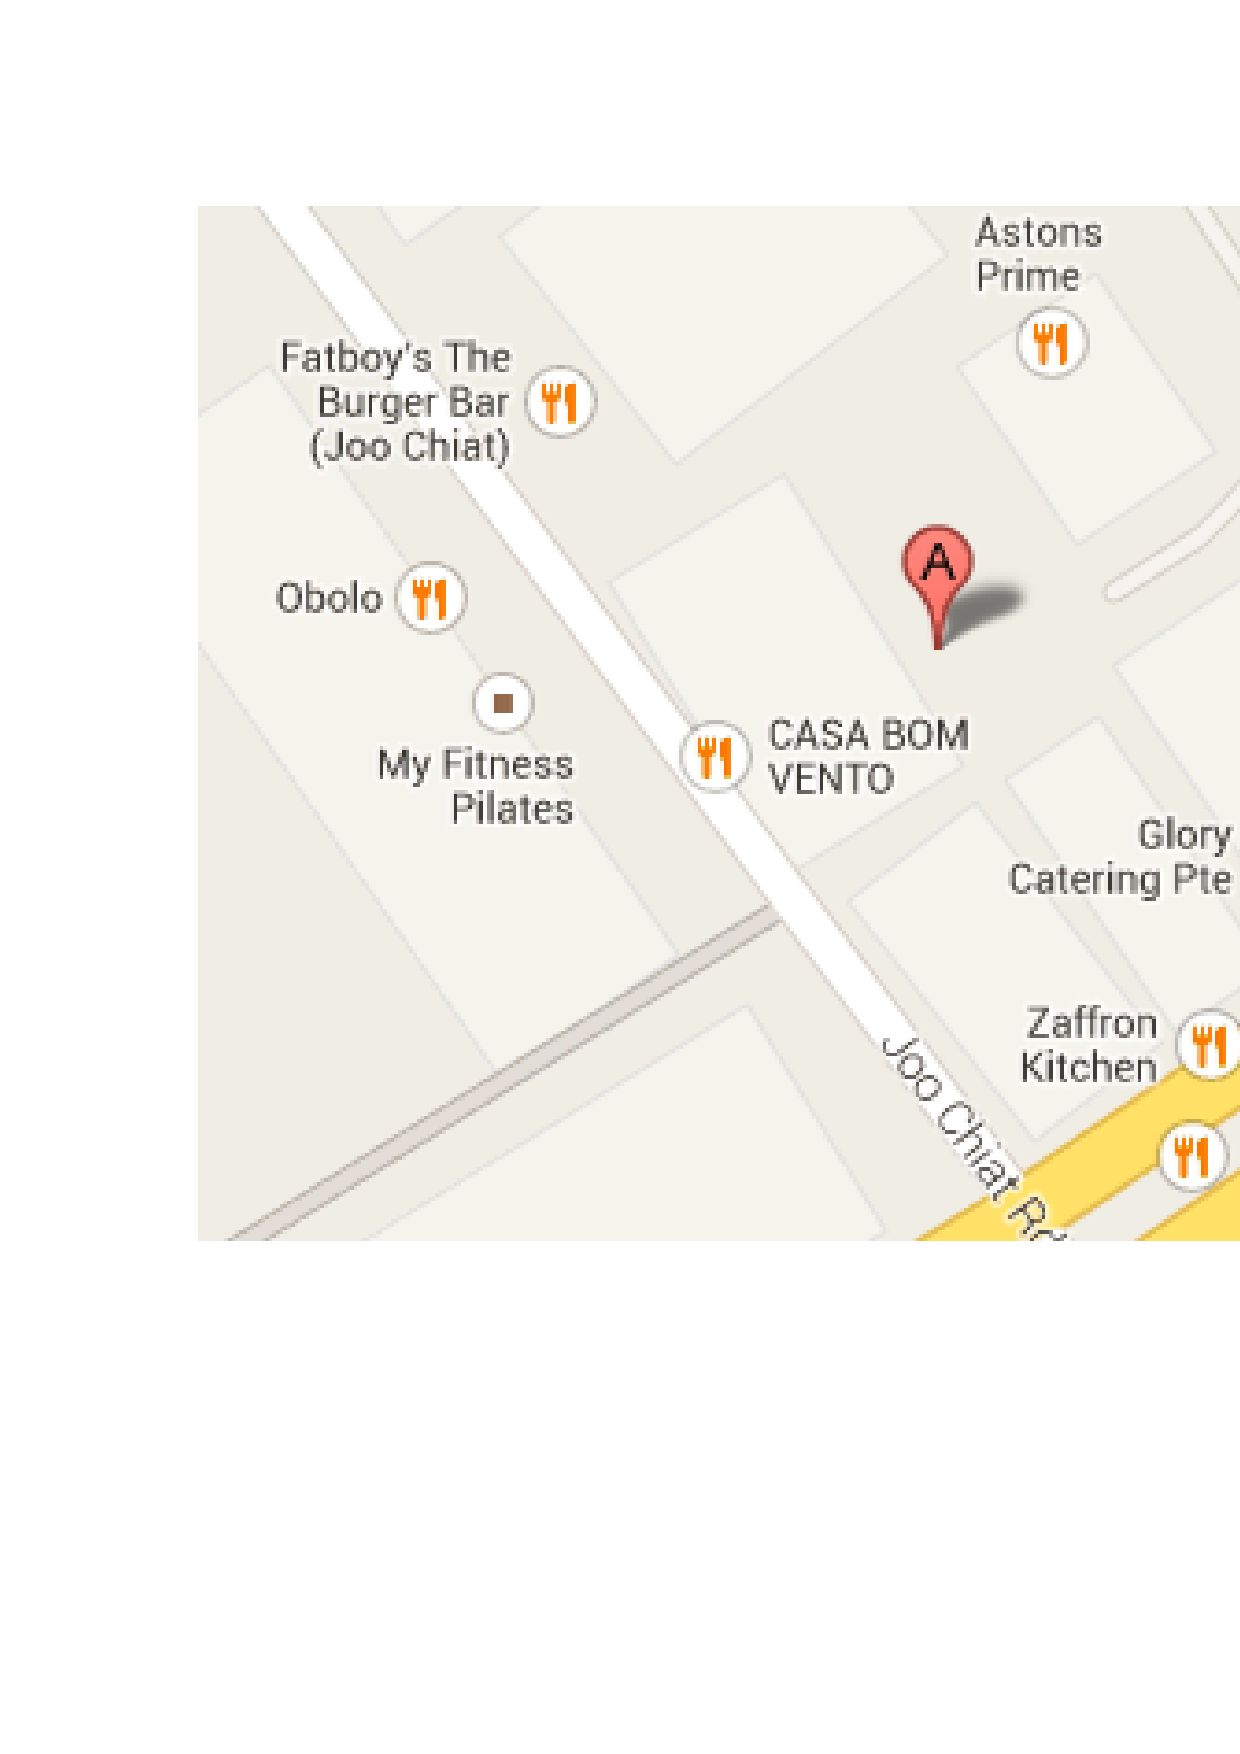
\includegraphics[width=0.32\textwidth]{figures/1.pdf}
	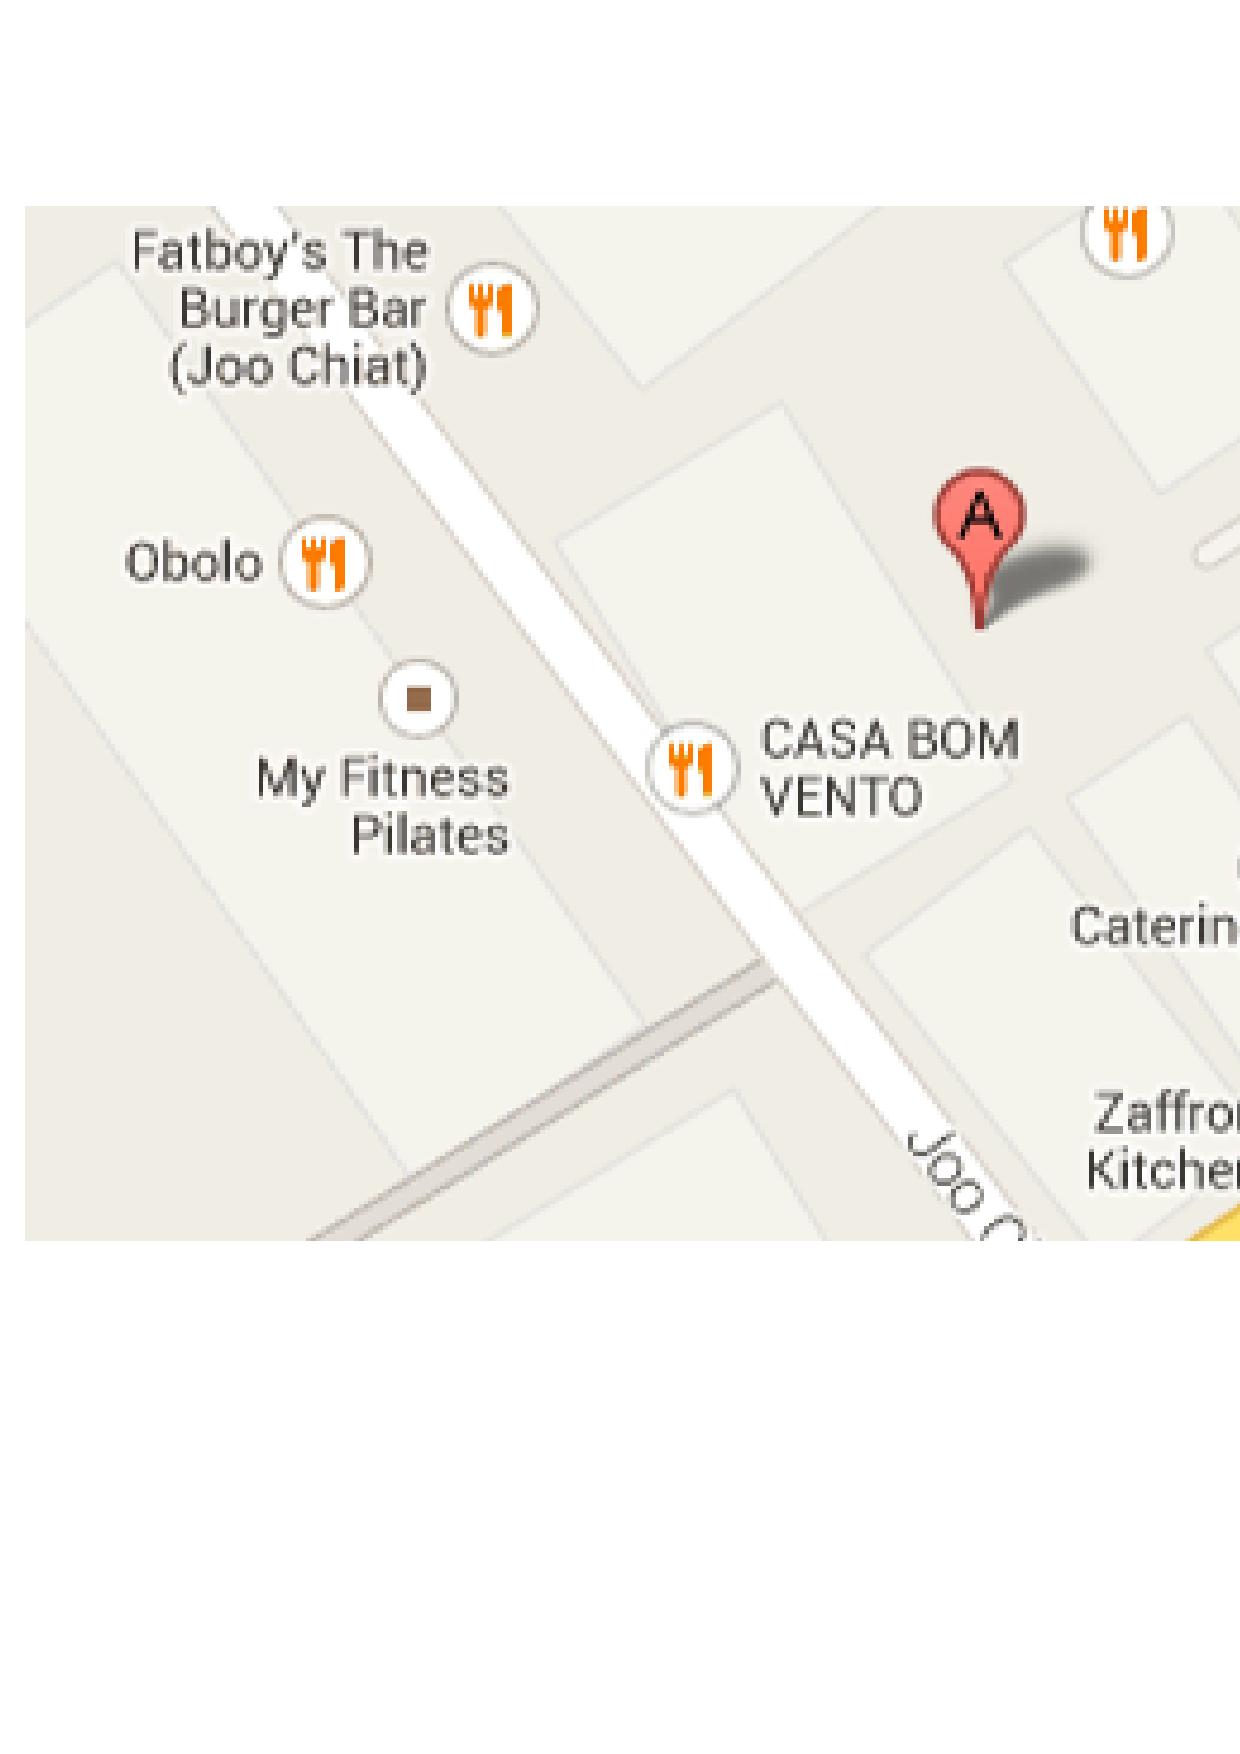
\includegraphics[width=0.32\textwidth]{figures/2.pdf}
	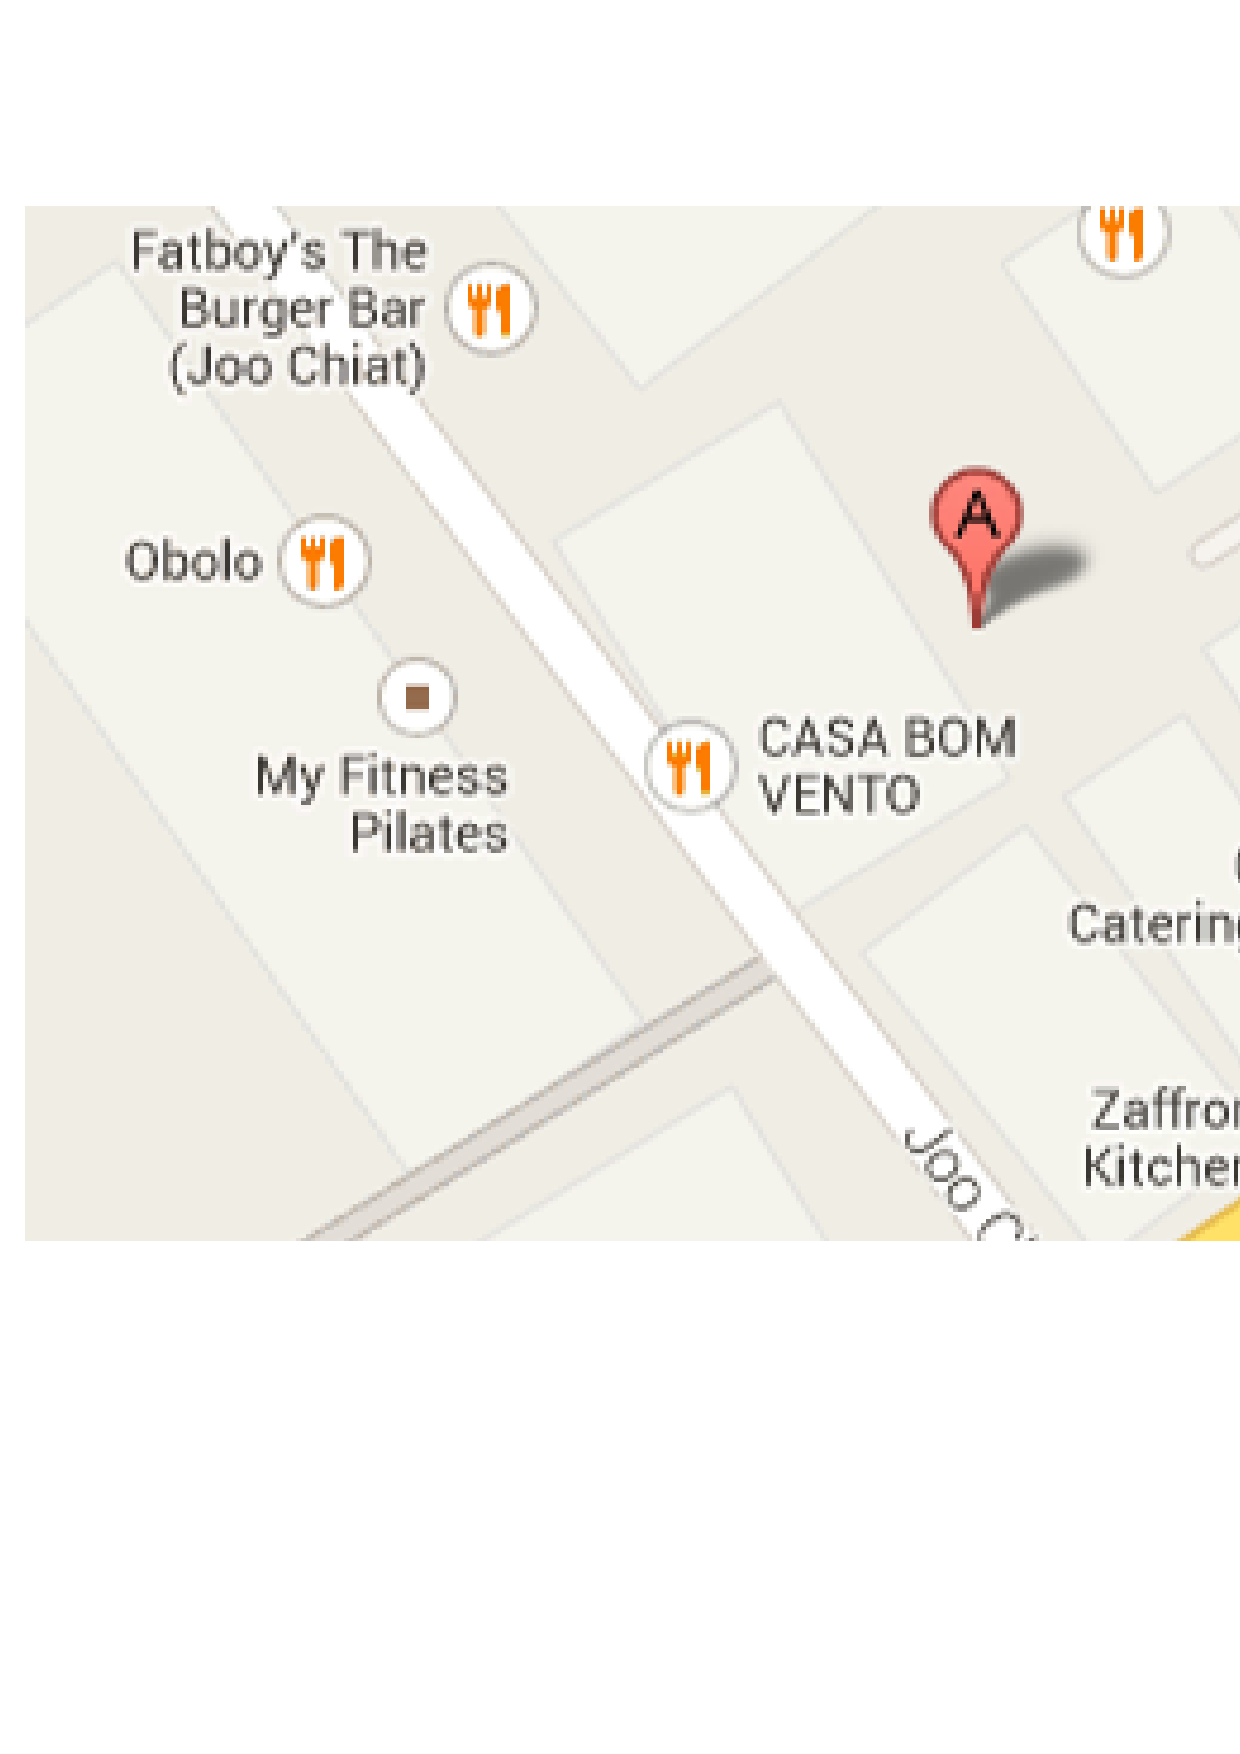
\includegraphics[width=0.32\textwidth]{figures/3.pdf}
	\includegraphics[width=0.32\textwidth]{figures/4.pdf}
	\includegraphics[width=0.32\textwidth]{figures/5.pdf}
	\caption{\textit{Local Transfer} and \textit{Cross-region Transfer} performances in terms of RMSE; Each sub-figure is a about region, and each cluster is either a \textit{Local Transfer} (LT) or a \textit{Cross-region Transfer} (CT).}
	\label{fig:transfer}
\end{figure*}
Also, we present the results of both \textit{Local Transfer} (LT) and \textit{Cross-region Transfer} (CT) in Figure~\ref{fig:transfer}.
It can be concluded from each sub-figure that our methods achieve the similar RMSE with the HAM without explicitly using historical data for links in target areas.
Also, we can find that when the two regions are similar to each other, 
then when we cross-region transfer one to another the performance is still good. 
Sometimes, even our CT methods can achieve very similar results then HAM without using any historical data on the predicted areas, such as ``Manhattan'' $\rightarrow$ ``Queens'' in the last sub-figure.
Apart from that, we found that a larger region like ``Manhattan'' which contains various kinds of links will have better CT performance than other regions.
Whereas, neural network model is relatively unstable. 
As for different prediction models, we conclude that our proposed CTPM performs substantially better than other classic feature-based methods.

%\section{Conclusion}
%In this paper,
%we study a both challenging and significant scenario of traffic prediction, which is to predict the future speed of a given road link but without its historical data. 
%We first extracted various spatial features to represent the geographical information of each links together with their temporal features,
%and then we design several feature-based transfer prediction models.
%Also, we proposed a novel two stage prediction model which clusters the links by their spatial features with regularization of their temporal similarities.
%%Experimental results show that our methods can achieve very close performance to models like HAM, without using any historical data of the predicted areas.
%



\bibliographystyle{aaai}
\bibliography{aaai}

\end{document}
